

\documentclass[openright]{xmgr}
\usepackage{minted}
% Jeśli nowe rozdziały mają się zaczynać na stronach
% nieparzystych:
%\documentclass[openright]{xmgr}

%\defaultfontfeatures{Scale=MatchLowercase}
%\setmainfont[Numbers=OldStyle,Ligatures=TeX]{Minion Pro}
%\setsansfont[Numbers=OldStyle,Ligatures=TeX]{Myriad Pro}
% for fontspec version < 2.0
%\setmonofont[Scale=0.75]{Monaco}
\setmainfont[Numbers=OldStyle,Mapping=tex-text]{Minion Pro}
\setsansfont[Numbers=OldStyle,Mapping=tex-text]{Myriad Pro}

% Opcjonalnie identyfikator dokumentu
% drukowany tylko z włączoną opcją 'brudnopis':
\wersja   {wersja wstępna [\ymdtoday]}

\author   {Adrian Pieper}
\nralbumu {243\,677}
\email    {adrpieper@gmail.com.pl}

\title    {Adventure Maker - język dla terenowych gier RGP}
\date     {2017}
\miejsce  {Gdańsk}

\opiekun  {dr W. Bzyl}

% dodatkowe polecenia
%\renewcommand{\filename}[1]{\texttt{#1}}
\definecolor{stress}{cmyk}{0,1,0.13,0} % RubineRed
\definecolor{topic}{cmyk}{0.98,0.13,0,0.43} % MidnightBlue

\begin{document}

% streszczenie
\begin{abstract}
  W ramach pracy został zaprojektowany i zaimplementowany \textit{Adventure Maker} - język domenowy\footnote{Domain Specific Language - DSL - język programowania służący do rozwiązywania jednej klasy problemów} służący do opisu terenowych gier RPG\footnote{Role Playing Game - Gra fabularna \url{https://pl.wikipedia.org/wiki/Gra_fabularna}}. Implementacja wykorzystuje technologię \textit{Xtext} \cite{Xtext:2017:Doc}. Narzędzie \textit{Xtext} umożliwiło stworzenie podstawowej infrastruktury języka zawierającej między innymi linker i kompiler. Dodatkowo powstały język zintegrowany jest z \textit{IDE IntelliJ IDEA}\footnote{Zintegrowane środowisko programistyczne \url{https://www.jetbrains.com/idea/}}, co pozwala na podświetlanie, automatyczne uzupełnianie i sprawdzanie składni.
  
  Wygenerowane przez \textit{Adventure Maker} gry wykorzystują technologię NFC\footnote{Near Field Communication - wysokoczęstotliwościowy standard komunikacji krótkiego zasięgu \url{https://pl.wikipedia.org/wiki/Near_Field_Communication}} oraz GPS\footnote{Global Positioning System - globalny system nawigacji satelitarnej \url{https://pl.wikipedia.org/wiki/Global_Positioning_System}} w celu lokalizowania graczy zarówno w pomieszczeniach, jak i na otwartym terenie. 
  
  W projekcie zostały wykorzystane popularne narzędzia i biblioteki, z których najważniejsze to \textit{Gradle}\cite{Gradle:2017:Doc}, \textit{JUnit}\cite{JUnit:2017:Doc} i \textit{Dagger 2} \cite{Dagger2:2017:Doc}. Kod został napisany zgodnie z zasadami Clean Code \cite{CleanCode:2005}.
  
  Praca składa się z dwóch części: implementacji języka \textit{Adventure Maker} oraz szablonu aplikacji, wraz z przykładowym kodem gry. Całość kodu dostępna jest w publicznym repozytorium GIT (pod adresem \url{https://github.com/adrpieper/magisterka}). Przykładowa aplikacja oraz wtyczka do \textit{IDE IntelliJ IDEA} zostały udostępnione na stronie \url{https://adrpieper.github.io/magisterka}.
\end{abstract}

% słowa kluczowe
\keywords{Android, DSL, Xtext, Location-Based Game, RPG}

% tytuł i spis treści
\maketitle

% wstęp
\introduction

Sukces niedawno wydanej gry \textit{Pokemon GO} pokazał, że pomysł by gracz musiał poruszać się po fizycznym świecie jest strzałem w dziesiątkę. Okazuje się, że na gry tego typu znajduje się całkiem spora rzesza odbiorców, czego nie dało się nie zauważyć, gdyż grupy poszukiwaczy tytułowych pokemonów, spotkać można było niemal na każdym kroku. Gry terenowe, czyli aplikacje rozrywkowe, bazujące głównie na fizycznej pozycji gracza, stały się nowym trendem w dziedzinie rozrywki elektronicznej.

Pomimo sukcesu \textit{Pokemon GO}, gry terenowe nadal stanowią niewielką część rynku rozrywki elektronicznej. Moim zdaniem niewielka ilość aplikacji tego typu, wynika z braku odpowiednich narzędzi do ich tworzenia. Napisanie tego typu gier w tradycyjny sposób jest dość skomplikowane, a przez to kosztowne. Wykorzystanie technologii typu GPS, czy NFC wymaga od programisty wiedzy i znajomości specjalistycznego API oraz sprawia, że testowanie aplikacji jest utrudnione.

Zauważyłem, że spora część elementów gier terenowych jest wspólna, szczególnie jeśli ograniczyć się jedynie do gier RPG. Pomyślałem, że skoro gry tego typu opierają się na podobnych zasadach, powinny one zostać zdefiniowane tylko raz, w myśl zasady programowania - "nie powtarzaj się" \cite{CleanCode:2005}. W ten sposób można by odciążyć projektanta gry od szczegółów implementacyjnych, pozwalając mu skupić się w całości na tym co ważne, czyli zasadach i scenariuszu rozgrywki. Stwierdziłem, że napisanie tego typu gry powinno sprowadzać się jedynie do zdefiniowania miejsc, postaci oraz zasad obowiązujących w wirtualnym świecie. Postanowiłem więc sprawdzić, czy osiągnięcie takiego ideału jest w ogóle możliwe. Okazuje się, że tak, o ile tylko zastosuje się do tego odpowiednie podejście i narzędzia.

Sam pomysł umieszczenia warstwy wspólnej dla wielu aplikacji nie jest nowy. Istnieje wiele takich rozwiązań. Warstwę tą nazywa się frameworkiem lub silnikiem gry. Większość powstających obecnie gier osadzonych jest właśnie na tego typu rdzeniu. Brak jest natomiast narzędzia wyspecjalizowanego do tworzenia konkretnego typu gier, jakimi są terenowe gry RPG.

Moim celem nie było stworzenie niesamowicie grywalnej, ani popularnej gry. Chciałem pokazać, na ciekawym moim zdaniem przykładzie gier terenowych, jak można rozwiązać problem "wynajdywania koła na nowo" wykorzystując własny język domenowy. Ponieważ wszystkie niezbędne w grze elementy są już zaimplementowane, \textit{Adventure Maker} pozwala na implementację gry przez osobę niebędącą programistą. Składnia języka jest przyjazna dla osoby zaznajomionej z tematyką gier RPG i nie wymaga znajomości, ani żadnego języka programowania ogólnego przeznaczenia, ani żadnych dodatkowych technologii.

Aby osiągnąć ten cel skorzystałem z popularnych i sprawdzonych narzędzi i rozwiązań. Do implementacji samego języka użyłem frameworka \textit{Xtext} oraz języka \textit{Xtend} \cite{Xtend:2017:Doc}. Framework dostarcza na podstawie gramatyki języka całą infrastrukturę języka zawierającą elementy takie jak: parser, linker, typechecker, compiler. Dodatkowo pozwala na integrację zaprojektowanego języka z popularnymi IDE: \textit{Eclipse} oraz \textit{IntelliJ IDEA}. 

\textit{Xtend} jest językiem programowania wywodzącym się i składniowo zbliżonym do Java, który został zaprojektowany, aby wyeliminować kilka wad tego języka. Zawiera elementy niedostępne w Java oraz upraszcza niektóre struktury pozwalając na pozbycie się niepotrzebnego kodu. Kodem wynikowym dla języka \textit{Xtend} jest Java, a nie kod binarny. Mamy tu więc do czynienia z transpilacją, czyli przetłumaczeniem jednego kodu źródłowego na inny. Wykorzystanie \textit{Xtend} jest zalecanym sposobem implementacji generatorów dla języków domenowych tworzonych przy użyciu \textit{Xtext}. Główną zaletą języka \textit{Xtend}, w kontekście pisania generatorów kodu, są szablony, które nie są dostępne w języku Java.

Aplikację napisałem za pomocą \textit{AndroidSDK} \cite{AndroidSDK:2017:Doc}. Jest to zestaw standardowych narzędzi programisty umożliwiający tworzenie aplikacji na platformę Android w języku Java. Przy wykorzystaniu \textit{AndroidSDK} zalecane jest użycie \textit{Gradle} \cite{Gradle:2017:Doc} - narzędzia służącego do automatyzacji budowania projektów informatycznych. Do jego zadań należą między innymi:
\begin{itemize}
\item Zarządzanie zależnościami
\item Automatyzacja testów
\item Budowanie i instalacja aplikacji
\end{itemize}
Wraz ze specjalnie zaprojektowanym pluginem, \textit{Gradle} stanowi obowiązkowy element każdego projektu związanego z systemem Android.

Do testów wykorzystałem biblioteki \textit{JUnit} \cite{JUnit:2017:Doc} oraz \textit{Mockito} \cite{Mockito:2017:Doc}. \textit{JUnit} służy pisania testów jednostkowych dla programów napisanych w języku Java. \textit{Mockito} umożliwia tzw. Mockowanie\footnote{Technika testowania polegająca na podmianie obiektu na jego atrapę \url{https://pl.wikipedia.org/wiki/Atrapa_obiektu}}.  Główną zaletą \textit{Mockito} jest bardzo wygodne API, tworzące swego rodzaju wewnętrzny DSL.

Aby móc zapanować nad zależnościami pomiędzy klasami wykorzystałem bibliotekę \textit{Dagger 2}.
Istnieje wiele bibliotek umożliwiających DI\footnote{Dependency Injection - wstrzykiwanie zależności \url{https://en.wikipedia.org/wiki/Dependency_injection}}, jednak \textit{Dagger 2} cieszy się największą popularnością wśród programistów systemu \textit{Android}. Jego główną zaletą jest rozstrzyganie zależności w czasie kompilacji oraz generacja kodu. Dzięki temu można wykryć wady projektu, takie jak zależności cykliczne jeszcze przed uruchomieniem aplikacji. Dodatkowo wygenerowany kod jest o wiele szybszy niż refleksja, czyli typowe rozwiązanie czasu wykonania. Jest to bardzo ważna cecha w przypadku aplikacji na urządzenia mobilne, ponieważ posiadają one stosunkowo ograniczone zasoby. 

\chapter{Przegląd istniejących rozwiązań}

W pracy postawiłem sobie na celu stworzenie języka domenowego pozwalającego na pisanie terenowych gier RPG. Cele postawione przed tym językiem są typowe dla frameworku - udostępnić narzędzie do przyjaznego rozwiązywania problemów określonej klasy. Nowy jest natomiast obszar w jakim działać będzie język, czyli terenowe gry RPG.

Tematyka pracy obejmuje więc, cztery pozornie niezwiązane ze sobą tematyki jakimi są gry terenowe, gry RPG, frameworki oraz języki domenowe. Ten rozdział ma na celu zaprezentowanie istniejących rozwiązań w każdej z tych dziedzin.

\section{Gry terenowe}

Rozwój technologii mobilny sprawił, że od paru lat na rynku rozrywki elektronicznej pojawił się całkiem nowy pomysł - gry terenowe. W grach tych zrezygnowano ze znanego z tradycyjnych gier wirtualnego świata na rzecz tzw. rzeczywistości rozszerzonej. W grach terenowych gracz nie steruje już postacią za pomocą myszki, czy klawiatury, lecz jest zmuszony do fizycznego przemieszczania się po rzeczywistym świecie. Lokalizacja gracza zostaje przeniesiona do świata gry za pomocą technologii takiej jak np. GPS. Mapa po której porusza się gracz jest więc mapą znaną z lekcji geografii. Elementami które sprawiają, że świat gry nazywamy rzeczywistością rozszerzoną, są pojawiające się w grze, a nie istniejące w rzeczywistości, obiekty lub postaci, które wpływają w jakiś sposób na przebieg rozgrywki.

Doskonały przykładem gry terenowej jest \textit{Pokemon GO}. Jest to gra, której premierę ciężko było przeoczyć. Gra zyskała olbrzymią popularność w zaledwie kilka dni, czego efektem były tłumy graczy szturmujących parki i place. Tam właśnie ukrywały się tytułowe Pokemony, których szukanie i kolekcjonowanie, są kluczowymi elementami rozgrywki.

Inny pomysł na wykorzystanie lokalizacji gracza mieli twórcy gry Landlord. Gra przenosi koncepcje znale z popularnej gry Monopoly do świata rzeczywistego. Cel gry pozostał niezmieniony, jest nim oczywiście inwestowanie w nieruchomości. Nie znajdziemy tam natomiast planszy, pionków, ani kostki. Gracze Landlord, w celu dokonywania wirtualnych zakupów, zmuszeni są do podróżowania po rzeczywistym świecie.

\section{Gry RPG}

Gry RPG, inaczej gry fabularne, są to gry w których gracze wcielają się w rolę fikcyjnych postaci poruszających się po fikcyjnym świecie.  Celem graczy jest zazwyczaj ukończenie jakiegoś scenariusza, bądź też po prostu osiągniecie określonego celu np. zdobycie jakiegoś przedmiotu, danej ilości złota lub rozwój postaci do konkretnego poziomu. Istnieją też gry otwarte, w których gracz nie ma żadnego narzuconego celu, a jedynie przemierza fikcyjny świat ze znanej tylko sobie motywacji. Tradycyjnie grę tego typu rozgrywa się w wyobraźni graczy. Jeden z graczy wciela się wtedy w tzw. mastera gry. Zadaniem mastera jest prowadzenia graczy przez świat gry poprzez opowiadanie pewnej historii oraz zadawanie pytań. Master przedstawia graczom jak wygląda sytuacja, w której znajdują się ich postacie oraz prosi ich o podjęcie decyzji, dotyczącej zachowania się postaci w danej sytuacji. Gracze podejmują decyzję, po czym master gry określa z jakimi skutkami się ona wiąże i przechodzi do dalszej opowieści. Aby zachować pewną spójność gry, master podejmuje decyzję w oparciu o ustalony zbiór zasad (tzw. mechanikę gry), zazwyczaj efekt podjętej decyzji zależy też od rzutu kością.

Oprócz tradycyjnej odmiany gier fabularnych powstały tej ich planszowe oraz komputerowe odmiany. W grach tych nie już mastera, a jego rolę przejmuje z góry narzucony scenariusz oraz ścisłe zasady. 

Jednym z najpopularniejszych przykładów planszowych gier RPG jest Magia i Miecz. Gracze wybierają w niej jedną z kilkudziesięciu postaci. Celem gry jest dostanie się do tzw. Korony Władzy. Aby móc tego dokonać muszę rozwinąć umiejętności swoich postaci. Jest to możliwe poprzez wyciąganie kart przygód, które zawierają opis sytuacji, w której znalazł się gracz. 

W świecie gier komputerowych, RPG osiągnęły niekwestionowany sukces. Wydanych tytułów są całe dziesiątki i nie sposób ich tutaj wymienić. Dodatkowo, warto zwrócić uwagę, że typowe elementy tych gier takie jak rozwój i statystyki postaci przedostały się już do prawie każdego gatunku gier komputerowych.

\section{Domain Specific Language (DSL)}

Domain Specific Languages \cite{DSL:2017}, czyli języki domenowe, projektowane są z myślą o ściśle określonym i z reguły bardzo wąskim zastosowaniu. W odróżnieniu od języków programowania ogólnego przeznaczenia, języki domenowe nie nadają się do rozwiązania większości problemów informatycznych. Sprawdzają się natomiast świetnie w dziedzinie, do której zostały zaprojektowane Dzięki ograniczeniu się jedynie do wąskiej grupy zastosowań, możliwe jest tworzenie języków, które są zrozumiałe dla osób będących ekspertami w danej dziedzinie. Języki domenowe należą zazwyczaj do języków deklaratywnych, gdyż skupiają są wokół tego co, a nie w jaki sposób, chce osiągnąć programista.

Języki domenowe ze względu na sposób ich implementacji można podzielić na dwie grupy:
\begin{itemize}
\item Języki wewnętrzne (Internal DSL)
\item Języki zewnętrzne (External DSL)
\end{itemize}

\subsection{Internal DSL}

Internal DSL to język stworzonych w ramach innego istniejącego już języka ogólnego przeznaczenia. Technicznie rzecz biorąc jest to zazwyczaj zbiór klas udostępniających wygodny dla programisty, dający wrażenie pisania w innym języku zbiór metod. Klasy te umieszcza się w bibliotece, którą możemy użyć do rozwiązania ściśle określonego problemu. Główną cechą takich bibliotek jest wyraźne nastawienie na udostępniany interfejs, a nie samą implementacje. O jakości takiego rozwiązania świadczy nie tyle wydajność jego działania, lecz łatwość użycia. Biblioteki takie pozwalają programiście na bardziej czytelne, prostsze i zwięzłe wyrażenie jego intencji. Przykładami taki języków są np. język asercji z biblioteki \textit{AssertJ} lub  biblioteka \textit{Mockito}. 

\subsection{External DSL}

External DSL to język domenowy z prawdziwego zdarzenia. Język taki posiada ściśle określoną gramatykę i od początku jest projektowany w określonym celu. Nie stanowi on części innego języka, chodź często z potrafi z nim współpracować. Przykładem takiej współpracy może być np. komunikacja z bazą danych, gdzie kod programu (napisany np w języku Java), wywołuje pewne zapytanie w języku SQL. Przykładami zewnętrznych języków domenowych są:
\begin{itemize}
	\item SQL - język służący do obsługi relacyjnych baz danych
	\item CSS - język służący do definiowania stylu stron internetowych 
	\item HTML - język służący do definiowania struktury strony internetowej
\end{itemize}

\section{Frameworki}

Frameworki są doskonałym przykładem korzyści jakie niesie ze sobą popularna zasada \textit{Clean Code} \cite{CleanCode:2005} - DRY (Don't Repeat Yourself), czyli nie powtarzaj się. 
Twórcy frameworków  wychodzą z założenia, że projekty informatyczne można z powodzeniem podzielić na pewne grupy. Projekty informatyczne należące do takiej grupy bywają do siebie tak podobne, że zazwyczaj łatwiej jest wskazać cechy wspólne niż różnice. Ideą frameworka jest implementacja wszystkich elementów wspólnych w jednym miejscu i udostępnienie programistom-użytkownikom frameworka przyjaznego interfejsu do implementacji tych różnic. Programista jest więc, ograniczony pewnymi ramami, w których musi mieścić się jego aplikacja, stąd nazwa takiego narzędzia.

Dobrym przykładem takiej grupy są aplikacje webowe.Wszystkie udostępniają pewien interfejs w postaci stron html, przechowują dane w bazach (zazwyczaj relacyjnych) i komunikują się z użytkownikiem za pomocą protokołu HTTP. Elementem różniącym te aplikacje jest ich wygląd i funkcjonalność. 

Z uwagi na fakt, że gry RPG są bardzo popularne, a jednocześnie do siebie bardzo podobne, naturalnym wydaje się stworzenie oprogramowania pozwalające na łatwe tworzenie takiego typu gier. Narzędzie \textit{RPG Maker} \cite{RPGMaker:2017:Doc} pozwala na proste wytwarzanie dwuwymiarowych gier RPG. Według twórców, tworzenie gier przy pomocy \textit{RPG Maker}, jest możliwe bez jakiejkolwiek wiedzy na temat programowania, jednocześnie dając bardzo duże możliwości doświadczonym użytkownikom. Oprogramowanie udostępnia przyjazne GUI, dzięki któremu można tworzyć w pełni funkcjonalne gry i to na wiele różnych platform. Jedynym, ale bardzo istotnym ograniczeniem jest ściśle narzucony gatunek gier. Jednak właśnie to ograniczenie pozwoliło na stworzenie narzędzia jednocześnie tak prostego i funkcjonalnego. 

Warto wspomnieć tu również o istnieniu narzędzi pozwalających na łatwe tworzenie nawet zaawansowanych gier mobilnych i to dowolnego typu. Takim oprogramowanie jest np. Unity \cite{Unity3D:2017:Doc}. Unity udostępsnia przyjazne GUI, które pozwala na tworzenie świata gry. Elementy fizyki takie jak grawitacja, są już w pełni zaimplementowane w silniku gry. Programista musi natomiast jedynie pamiętać o nadaniu obiektom odpowiednich cech takich jak np. masa. Logikę gry można zaimplementować w jednym z dwóch języków UnityScript oraz C\#. UnityScript jest językiem o składni bardzo zbliżonej do JavaScript, natomiast C\# to popularny obiektowy język programowania czerpiący wszystko co dobre z Java i C++. Użycie powszechnie znanych języków oraz wieloplatformowość z pewnością przyczyniły się do olbrzymiej popularności, którą cieszy się Unity.


\chapter{Wymagania języka \textit{Adventure Maker}}

Jednym z pierwszym kroków, jakie należy podjąć przed przystąpieniem do projektowania oprogramowania jest analiza wymagań. Andventure Maker umożliwia tworzenie gier terenowych o narzuconych z góry, dość wąskich i specyficznych ramach, typowych dla tradycyjnych gier RPG. Napisana w nim gra polega głównie na rozwoju postaci poprzez odwiedzanie lokacji, podejmowanie decyzji oraz pokonywanie przeciwników. Postać sterowana przez gracza zdobywa punkty doświadczenia, dzięki którym gracz może rozwijać postać w wybranym przez siebie kierunku. 

Wymagania, jakie postawiłem przed \textit{Adventure Maker} można podzielić na funkcjonalne i niefunkcjonalne.

\section{Funkcjonalne}
Do wymagań funkcjonalnych należą:
\begin{itemize}
\item Język DSL zawierający elementy:
\subitem - Klasy Postaci
\subitem - Przedmioty
\subitem - Lokacje
\subitem - Przygody
\subitem - Przeciwnicy
\item Integracja ze środowiskiem \textit{IntelliJ IDEA}
\item Kompilacja aplikacji na podstawie pliku DSL 
\end{itemize}

Zbiór elementów wchodzących w skład zaprojektowanego języka DSL został przeze mnie wybrany arbitralnie, w taki sposób, żeby zawierał minimum niezbędne do zaprojektowania gry. Chciałem, aby zaprojektowany język był jednocześnie prosty, ale i pozwalający na implementację nawet dość zawiłej logiki. Oczywiście RPG z prawdziwego zdarzenia powinien być bardziej rozbudowany. Uznałem jednak, że dodanie elementów takich jak np. misje zbędnie skomplikowały by język. Elementy te prawdopodobnie pojawią się, w przypadku wydania kolejnej wersji \textit{Adventure Maker}. Niemniej jednak implementacja stworzona w ramach tej pracy obejmować będzie jedynie wyszczególnione punkty.

W celu ułatwienia edycji kodu warto udostępnić użytkownikowi przyjazne IDE. Na szczęście narzędzia takie już istnieją i nie musiałem projektować ich od zera. Popularne narzędzia programistyczne pozwalają na rozszerzanie ich funkcjonalności poprzez tzw. wtyczki, czyli oprogramowanie, które doinstalowuje się do już istniejącego IDE. Postanowiłem więc, że udostępnię obsługującą język \textit{Adventure Maker} wtyczkę do IDE \textit{IntelliJ IDEA}. Wybrałem to środowisko z kilku powodów:
\begin{itemize}	
\item jest darmowy w wersji Community,
\item udostępnia integracje z Android SDK,
\item jest wspierany przez \textit{Xtext} i \textit{Xtend}.
\end{itemize}

Przyjazna edycja kodu to za mało, aby język był funkcjonalny. Użytkownikowi należy udostępnić możliwość kompilacji kodu. W tym przypadku będzie to transkompilacja, ponieważ kodem wyjściowym nie będzie kod binarny, a kod Java. Na podstawie wygenerowanego oraz dostarczonego kodu musi być możliwa kompilacja gotowej aplikacji, bez konieczności dopisywania ani jednej linii dodatkowego kodu. 

\section{Niefunkcjonalne}
Do wymagań niefunkcjonalnych należą:
\begin{itemize}
	\item Tworzenie gier RPG bez znajomości technologii i języków programowania ogólnego przeznaczenia
	\item Wykorzystanie darmowych narzędzi
	\item Ukrycie szczegółów implementacyjnych GPS i NFC przed użytkownikiem języka
\end{itemize}

Podstawowym założeniem \textit{Adventure Maker} jest udostępnienie możliwości tworzenia gier osobom będącym laikami jeśli chodzi o programowanie i technologie IT. Abym mógł w ogóle udostępnić im ten język, ważne jest wykorzystanie darmowych narzędzi.

Język \textit{Adventure Maker} został zaprojektowany tak, aby twórca gry mógł traktować technologie NFC i GPS w sposób bardzo zbliżony nie zważając na ich  całkowicie odmienną techniczną implementację. Z jego punktu widzenia zarówno pomieszczenie oznaczone tagiem NFC, jak i współrzędne geograficzne, stanowią po prostu lokację, w której gracza mogą spotkać dowolnego typu przygody. 

\chapter{Projekt Interfejsu Aplikacji}
Ważnym elementem oprogramowania jest jego graficzny interfejs użytkownika \footnote{GUI - Graphical User Interface - Graficzny interfejs użytkownika}. W przypadku języka do tworzenia gier można mówić o dwóch rodzajach GUI. Pierwszym jest interfejs środowiska służącego do edycji kodu, drugim interfejs gier napisanych w tym języku.

Jako, że \textit{Adventure Maker} został zrealizowany jako wtyczka do istniejącego IDE, sprawa jego GUI jest rozwiązana. IDE \textit{IntelliJ IDEA} dostarcza bardzo wygodny i dopracowany interfejs użytkownika, a dostarczona przeze mnie wtyczka wykorzystuje jego możliwości. 

Język nie pozwala twórcy gry na dostosowanie interfejsu do swoich potrzeb. Tak więc, jako jego projektant, postanowiłem przygotować interfejs prosty, a zarazem uniwersalny i neutralny względem klimatu gry. GUI jest podzielone na trzy części:
\begin{itemize}
	\item Menu początkowe
	\item Tryb Zwiedzania
	\item Tryb Przygody
\end{itemize}
\section{Menu początkowe}
Ekran pozwala na wybór typu postaci, jaką dany gracz ma zamiar kontrolować. Został podzielony na dwie części: listy klas postaci oraz szczegółów wybranej klasy. Szczegóły zawierają nazwę klasy oraz informacje o jej statystykach.

\section{Tryb Zwiedzania}
Ekran zwiedzania wyświetlany jest przez cały czas, w którym gracz porusza się pomiędzy lokacjami w poszukiwaniu przygód. 

Tryb zwiedzania zawiera dosyć dużo informacji, dlatego też został podzielony na następujące części: 
\begin{itemize}
	\item Przegląd postaci
	\item Umiejętności
	\item Przedmioty
\end{itemize}
Pomiędzy widokami gracz może nawigować swobodnie, przeciągając je w lewo lub w prawo.
\subsection*{Przegląd postaci}
Przegląd postaci zawiera informacje o ilości i poziomie doświadczenia sterowanej przez gracza postaci. Dodatkowo wyświetla też statystyki uwzględniające bonusy otrzymane z używanych przedmiotów.
\subsection*{Umiejętności}
Ekran udostępnia drzewko umiejętności oraz dwa przyciski \textit{Reset} oraz \textit{OK}. Drzewko służy zarówno do przeglądania posiadanych, jak i odblokowywania nowych umiejętności. Przycisk \textit{Reset} przywraca graczowi rozdane punkty umiejętności, natomiast przycisk \textit{OK} zatwierdza ich wybór.
\subsection*{Przedmioty}
Sekcja zawiera wszystkie posiadane przez gracza przedmioty. Te używane aktualnie znajdują się w górnej części ekranu, natomiast pozostałe w dolnej, zwanej plecakiem. Dodatkowo na środku wyświetlana jest suma bonusów do statystyk uzyskanych z noszonych przedmiotów.
\section{Tryb Przygody}
Gracz nie ma swobodnego dostępu do tej części interfejsu. Jest ona wyświetlana dopiero w momencie znalezienia się gracza w lokacji zawierającej jakąś przygodę.

Tryb przygody zawiera kilka ekranów, z których każdy odpowiedzialny jest za wyświetlenie konkretnego zdarzenia. Gracz nie może swobodnie nawigować pomiędzy nimi. Dostępne GUI zależne jest od sytuacji, w której znajduje się postać gracza.
\subsection*{Decyzja}
Ekran pozwala graczowi na podjęcie decyzji związanej z dalszym przebiegiem \textit{Przygody}. Zawiera jedynie pole wyświetlające pytanie skierowane do gracza oraz listę decyzji w postaci przycisków. 
\subsection*{Walka}
Widok walki służy do wyświetlania oraz sterowania przebiegiem starcia pomiędzy postacią gracza, a dowolnym przeciwnikiem. Interfejs wyświetla nazwę przeciwnika, kolorowe paski zawierające informacje o punktach życia postaci i przeciwnika oraz o punktach many\footnote{W fantastyce rodzaj energii stosowanej np. do rzucania zaklęć \url{https://pl.wikipedia.org/wiki/Mana_(fantasy)}} gracza. W dolnej części znajdują się przyciski akcji pozwalające na użycie standardowego ataku lub dowolnej umiejętności.
\subsection*{Komunikat}
Ekran komunikatu składa się z dwóch części: wyświetlanej informacji oraz przycisku \textit{OK}, którym gracz potwierdza, że zapoznał się z komunikatem. Informacja najczęściej wyświetlana jest w prostym oknie tekstowym, jednak w niektórych przypadkach konieczne jest użycie elementów bardziej rozbudowanych. Jest tak na przykład w przypadku okna wyświetlanego pod koniec przygody, zawierającego między innymi wykaz zdobytych przez gracza przedmiotów w postaci listy.

\chapter{Architektura Języka i Aplikacji}

\textit{Adventure Maker} składa się z dwóch projektów. Pierwszy odpowiedzialny jest za implementacje języka. Drugi projekt, to szkielet aplikacji na system Android, będący bazą pod wszystkie gry pisane w \textit{Adventure Maker}. 

\section{\textit{Adventure Maker} DSL} 
Projekt powstał w celu implementacji gramatyki i generatora dla języka Andventure Maker. Projekt bazuje na narzędziu \textit{Xtext}\cite{Xtext:2017:Doc}, a produktem wyjściowym jest wtyczka do IDE \textit{IntelliJ IDEA} obsługująca zaprojektowany DSL. 

\subsection{Definicja Gramatyki} 

Gramatyka języka \textit{Adventure Maker} znajduje w pojedynczym pliku o nazwie "AML.xtext". Definicja w nim zawarta zawiera zarówno opis modelu syntaktycznego i semantycznego tworzonego języka. Innymi słowy zdefiniuje jaki tekst należy do języka oraz jak będzie on reprezentowany w pamięci komputera. \textit{Xtext} na podstawie tego pliku generuje między innymi parser, który sprawdzi, czy dany tekst poprawnym programem oraz zwróci jego reprezentacje w postaci drzewa obiektów.

\subsection{Generator Kodu}
Generator odpowiedzialny jest za wygenerowanie kodu (w tym przypadku kodu Java) na podstawie modelu semantycznego zwróconego przez parser w postacie drzewa obiektów. Generator został napisany w języku \textit{Xtend} i składa się z głównej klasy implementującej metodę \textit{doGenerate} oraz klas pomocniczych utworzonym w celu dekompozycji problemu na mniejsze części zgodnie z zasadą pojedynczej odpowiedzialności \cite{CleanCode:2005}.

\section{Aplikacja Android}
Ten projekt to standardowa aplikacja androidowa wykorzystująca \textit{AndroidSDK} rozbudowana o język \textit{Adventure Maker}, na podstawie którego generowana jest cześć kodu aplikacji.

Architektura projektu jest dość rozbudowana i można z niej wydzielić następujące moduły:

\begin{itemize}
	\item Standardowy Kod Aplikacji
	\item Zasoby
	\item Plik manifestu
	\item Pliki \textit{Grandle}
	\item Testy
	\item Wewnętrzy DSL
	\item Plik game.aml
	\item Wygenerowany Kod Implementujący Zasady Gry
	\item Testowy Kod Implementujący Zasady Gry
\end{itemize}

Pierwsze pięć elementów jest typowych dla aplikacji android, natomiast pozostałe są specyficzne i wynikają z zastosowania języka \textit{Adventure Maker}.

\subsection*{Standardowy kod aplikacji} 

Jest to bardzo rozbudowana, ale i najbardziej tradycyjna i oczywista część aplikacji. W jego skład wchodzą pakiety \textit{edu.ug.inf.am.*} umieszczone w folderze \textit{app/src/main/java}. Moduł jest odpowiedzialny za sposób działania i wygląd aplikacji. Korzysta z kodu Implementujący Zasady Gry oraz Zasobów. Została w nim umieszczona logika związana z systemem Android taka jak komunikacja z czujnikami NFC i GPS, czy obsługa interfejsu użytkownika. Dodatkowo kod odpowiada za elementy stałe dla każdej gry takie jak mechanizm walki i rozwoju postaci.

Kod został podzielony na warstwy i komponenty, co zostało odzwierciedlone w strukturze pakietów. 
Komponenty to zbiory klas realizujące wspólne zadanie. Ich struktura jest hierarchiczna tzn. w skład konkretnego komponentu wchodzą kolejne, odpowiedzialne za zadania bardziej sprecyzowane. Kompletną strukturę komponentów aplikacji przedstawie drzewo \ref{modules:tree}.

\begin{figure}[!tbh]
	\centering
	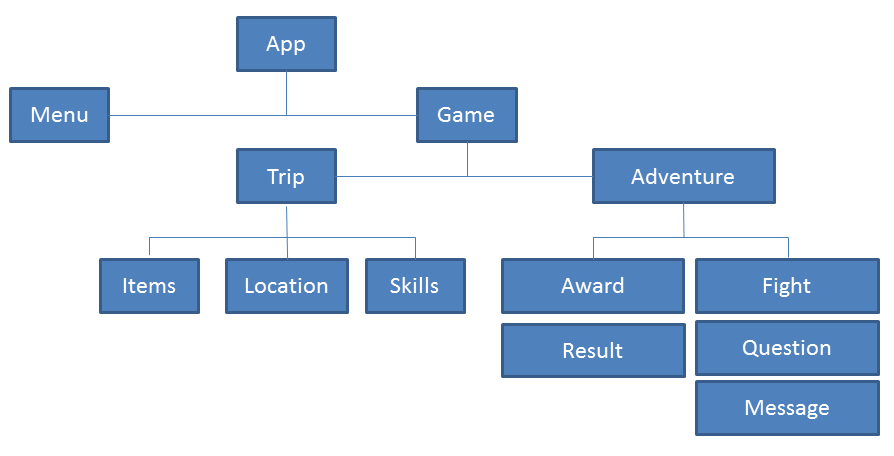
\includegraphics[width=1.0\hsize]{fig/modules_tree}
	\caption{Struktura komponentów aplikacji}
	\source{Własne opracowanie}
	\label{modules:tree}
\end{figure}

Wszystkie komponenty zostały zrealizowane w postaci pakietów o podobnej strukturze. W nich skład wchodzi po kilka pakietów-warstw zawierających bezpośrednio klasy realizujące funkcjonalność tych warstw. Dodatkowo pakiety, nie będące liśćmi w drzewie, zawiera pakiety-komponenty znajdującymi się niżej w hierarchii.

W kodzie wydzieliłem następujące warstwy i odpowiadające im nazwy pakietów:
\begin{itemize}
	\item Widok (view)
	\item Contoler (controller)
	\item Model (model,state)
	\item Logika (logic)
	\item Komponent (dagger)
\end{itemize}

Widok to warstwa odpowiedzialna za interfejs użytkownika. W jej skład wchodzą przede wszystkim klasy dziedziczące po \textit{Activity}, Fragment oraz View. W większości przypadków zadaniem klasy jest połączenie danych, udostępnianych przez warstwę kontrolera, z widokiem za pomocą dostępnego od niedawna w systemie \textit{Android} mechanizmu \textit{Data Binding}\cite{AndroidSDK:2017:Doc}.

Warstwa kontrolera odpowiada przede wszystkim za obsługę zdarzeń przychodzących z interfejsu użytkownika, oraz dostarczanie modelu danych dla widoku. Zajmuje się też modyfikacją danych. W prostych przypadkach modyfikuje je bezpośrednio, a w bardziej zaawansowanych deleguje to zadanie do warstwy logiki. Inną ważną odpowiedzialnością tej warstwy jest przełączanie pomiędzy widokami. 

Model odpowiada za przechowywanie danych w uporządkowany sposób. Hermetyzuje dane udostępniając zestaw metod dostępowych (\textit{gettery} i \textit{settery}). Ta warstwa została podzielona na dwa podtypy: model i stan. Modelem nazywam wszystkie klasy, których stan jest obserwowany przez widok (wzorzec obserwator). Stanem (State) nazywam klasy typu POJO \footnote{Plaid Old Java Object - prosty obiekt, nie zależny od zewnetrznego frameworku \url{https://pl.wikipedia.org/wiki/Plain_Old_Java_Object}}, których stan nie może być obserwowany, a ich jedynym zadaniem jest przechowywanie stanu aplikacji. 

Logika to warstwa odpowiadająca za wszelkie operacje wykonywane na danych, które nie powinny znaleźć się w warstwie kontrolera ze względu na zbyt duże skomplikowanie, bądź wagę kodu. Wydzielenie tego kodu do osobnych klas w połączeniu z testowaniem jednostkowym pozwala stworzyć kod, co do którego mamy pewność, że jego kluczowe aspekty działają prawidłowo. Usunięcie tego kodu z kontrolera jest zgodne z zasadą pojedynczej odpowiedzialności \cite{CleanCode:2005} i pozwala na jego użycie w wielu miejscach programu. 

Pakiet \textit{dagger} to miejsce w którym integrowane są wszystkie klasy należące do danego komponentu. W projekcie wykorzystano technikę wstrzykiwania zależności (DI), która pozwala na usunięcie bezpośrednich zależności pomiędzy klasami, aż do momentu ich integracji. Za wstrzykiwanie zależności w moim projekcie odpowiedzialna jest biblioteka \textit{Dagger 2}, stąd nazwa pakietu w którym to zadanie jest realizowane.

\subsection*{Zasoby}
Zasoby są elementem wspólnym dla każdej aplikacji. Tradycyjnie zostały umieszczone w folderze \textit{app/scr/main/res}. Tutaj definiuje się elementy takie jak layouty, ikonki, animacje itp. Większość zasobów stanowią pliki xml. Dostęp do zasobów możliwy jest z poziomu kodu aplikacji poprzez klasę R. Klasa ta jest generowana automatycznie, a jej skład wchodzi zestaw stałych, będących identyfikatorami odpowiednich zasobów. \textit{AndroidSDK} posiada wbudowany system zarządzania zasobami, który pozwala na przygotowanie konkretnego zasobu w kilku wersjach (np. różny layout dla kilku wielkości ekranów). Tak przygotowany zasób, jest dostępny pod pojedynczym numerem id, a o wybór odpowiedniej wersji dba system.

Większość zasobów stanowią layouty, z których znaczna część wykorzystuje \textit{Data Binding}. Mechanizm pozwala opisać logikę odpowiedzialną za wyświetlanie danych w sposób deklaratywny, przy pomocy języka \textit{xml}. \textit{AndroidSDK} generuje na jego podstawie specjalny kod, który będzie realizował to zadanie. 

\subsection*{Plik manifestu}
Plik manifestu jest elementem niezbędnym w każdej aplikacji androidowej. Znajduje się on w folderze \textit{app/scr/main}. W nim zadeklarowane są elementy takie jak identyfikator aplikacji, zbiór dostępnych aktywności, potrzebne uprawnienia, ikonę startową itp.

\subsection*{\textit{Gradle}}
\textit{Gradle} jest narzędziem służącym do budowania projektów, który stał się standardem w aplikacjach androidowych. W projekcie znajdują się 2 pliki \textit{Gradle}, jeden dla modułu aplikacji, drugi dla całego projektu, które zostały umieszczone odpowiednio w folderze "/app" i "/". W plikach \textit{Gradle} zdefiniowane jest struktura projektu, zadania związane z jego budowaniem oraz potrzebne zależności.

\subsection*{Testy}
Moduł testów odpowiedzialny jest za sprawdzenie, czy kod aplikacji działa prawidłowo. Ich  kod został umieszczony w folderze\textit{app/scr/test/java}. W jego skład wchodzą klasy, implementujące testy jednostkowe wszystkich ważnych elementów aplikacji. Kod testów wykorzystuje zewnętrzne biblioteki \textit{JUnit}, \textit{Mockito} i \textit{AssertJ}.

\subsection*{Wewnętrzy DSL}

W projekcie wykorzystałem zarówno wewnętrzny, jak i zewnętrzny język domenowy. Zastosowanie zewnętrznego DSL pozwala twórcy gry na opisanie świata gry w sposób przyjazny dla osoby znającej tematykę gier RPG.  Wewnętrzny DSL jest odpowiedzialny za dostarczenie wygodnego API do opisu zasad gry w języku Java, co znacznie uprościło zaimplementowania generatorów kodu.

Technicznie rzecz biorąc moduł stanowi on interfejs do komunikacji pomiędzy modułami Standardowy Kod Aplikacji, a Kodem Implementujący Zasady Gry. Zarówno dostarczone API, jak i implementacja modułu zostały zrealizowana w języku Java. Dlatego też nazywam go wewnętrznym językiem domenowym. W skład modułu wchodzą wszystkie klasy pakietów \textit{pl.aml.*}.

Istotną częścią tego modułu są klasy pozwalające na wygodne budowanie obiektów (tzw. \textit{Buildery}\footnote{Builder - Budowniczy  - wzorzec projektowy  \url{https://pl.wikipedia.org/wiki/Budowniczy_(wzorzec_projektowy)}}) oraz metody statyczne tworzące instancje tych klas. Różnicę pomiędzy kodem pisany z i bez wykorzystania wewnętrznego DSL zaprezentowałem w dodatku A.

\subsection*{Plik game.aml}
Plik znajduje się w folderze \textit{app/src/main/java}. Jest kluczowym elementem całego projektu, bo to właśnie w nim definiuje się w języku \textit{Adventure Maker} elementy związane z konkretną grą.

\subsection*{Wygenerowany Kod implementujący zasady gry}
Ten moduł znajduje się folderze \textit{app/aml-src} i zawiera kod wygenerowany automatycznie na podstawie pliku \textit{game.aml}. Kod ten implementuje szczegóły dotyczące konkretnej gry. Wykorzystuje API dostarczone przez Wewnętrzny Język DSL. Wygenerowany tu kod użyty jest w module Kod Aplikacji.

\subsection*{Testowy Kod implementujący zasady gry}
Ten moduł zawiera kod analogiczny do Wygenerowanego Kodu implementujący zasady gry, jest jednak napisany ręcznie. Kod został umieszczony w folderze \textit{app/test-src}. Moduł ten zastępuje kod generowany podczas testowania i rozwijania aplikacji i nie jest wykorzystywany w produkcie finalnym.

\chapter{Testy} 

W celu sprawdzenia poprawności działania stworzonego oprogramowania musiałem je przetestować. Na pierwszym miejscu postawiłem testy automatyczne, ponieważ są najbardziej praktyczne i wiarygodne. Testy automatyczne zaimplementowałem w postaci mockowanych testów jednostkowych za pomocą bibliotek \textit{JUnit} i \textit{Mockito}.

Niestety z przyczyn technicznych nie dało się pokryć testami automatycznymi wszystkich funkcjonalności. Z tego powodu część kodu została przetestowana w sposób manualny. Elementami przetestowanymi ręcznie są działanie modułu NFC oraz GPS. Do każdego z tych elementów przygotowałem scenariusz testowy, który następnie wykonałem. Sposób przeprowadzenia oraz wyniki tych testów zostały przedstawione poniżej.

\section{Testy automatyczne}
\subsection{Struktura testów}
Podczas  automatycznych testów jednostkowych testowałem z osobna działanie poszczególnych funkcji w oderwaniu od reszty systemu. Każdy test został podzielony na 3 sekcje, zawierające kod odpowiedniego typu:
\begin{itemize}
\item \textit{Given}
\item \textit{When}
\item \textit{Then}
\end{itemize}

W sekcji \textit{Given} został umieszczony kod implementujący warunki początkowe. Są to przede wszystkim linie kodu mockującego metody klas zależności klasy testowanej. Mogą to być też wywołania metod dostarczających jakieś dane. 

Sekcja \textit{When} składa się z pojedynczej linii. Jest to wywołanie testowanej metody na instancji testowanej klasy.

Sekcja \textit{Then} odpowiedzialna jest za sprawdzenie, czy metoda zachowała się w oczekiwany sposób. Zazwyczaj jest to kod składający się z kilku linii zawierających asercje. Asercje służą sprawdzeniu czy, ile razy i z jakimi parametrami zostały wywołane metody klas-zależności. Jeżeli funkcja zwraca jakiś wynik, za pomocą asercji testuje się, czy pokrywa się on z oczekiwanym.

\subsection{Wyniki}
Testy jednostkowe zostały uruchomione przy pomocy narzędzia \textit{Gradle} \cite{Gradle:2017:Doc}. Poniższe zestawienie pokazuje, że wszystkie testy przeszły pomyślnie.

\begin{figure}[!tbh]
	\centering
	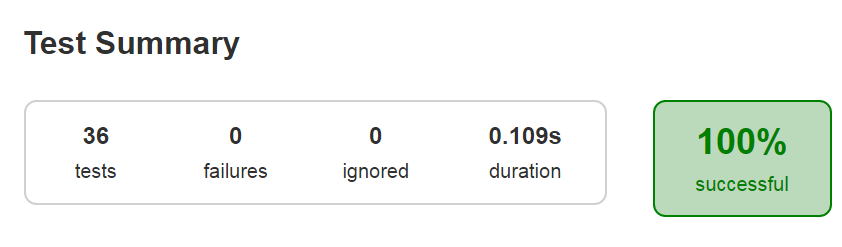
\includegraphics[width=1.0\hsize]{fig/test_summary}
	\caption{Podsumowanie testów}
	\source{Wygenerowane przez \textit{Gradle}}
\end{figure}

\section{NFC i GPS}

Testy funkcjonalność NFC i GPS zostały przeprowadzone ręcznie według poniższego scenariusza:

\begin{itemize}
  \item Przygotowanie pliku AML\footnote{Adventure Maker Language - rozszerzenie plików obsługiwane przez język \textit{Adventure Maker}}
  \item Kompilacja
  \item Sprawdzenie poprawności zachowania
\end{itemize}

\section{Plik AML}

Przygotowane pliki AML dla testu NFC i GPS są bardzo podobne. Oba składają się z przykładowej Klasy Postaci oraz dwóch Przygód i Lokacji. W obu przypadkach przygody polegają jedynie na wyświetleniu komunikatu. 

Różnica pojawia się w przypadku definicji Lokacji. W pliku przygotowanym dla GPS, są to dwa znajdujące się niedaleko od siebie obszary o promieniu 10 metrów. W przypadku NFC Lokacje zdefiniowane są przez odpowiednie znaczniki "Test1" i "Test2".

Kod \textit{Adventure Maker} przygotowany do przeprowadzenia obydwu testów znajduje się w załączniku.

\subsection{Sprawdzenie poprawności zachowania}

Poprawność działania modułów GPS i NFC została sprawdzona manualnie. W obu przypadkach sprawdziłem, czy wejście do odpowiedniej Lokacji uruchomi odpowiednie zdarzenie.

W przypadku testu GPS przeszedłem się z urządzenie wyposażonym w moduł GPS w odpowiednie miejsca. W przypadku NFC po prostu przyłożyłem telefon do odpowiednich znaczników. 

Oba testy zakończyły się sukcesem.  

\chapter{Pisanie gier w \textit{Adventure Maker}}
Pisanie własnej gry przy użyciu \textit{Adventure Maker} wymaga przygotowania środowiska pracy. W tym rozdziale zawarłem instrukcje dotyczące instalacji, konfiguracji i korzystania z potrzebnych narzędzi. 

\section{Konfiguracja środowika}

Aby móc korzystać z \textit{Adventure Maker} należy pobrać i zainstalować IDE \textit{IntelliJ IDEA}, JRE\footnote{Java Runtime Enviroment - środowisko uruchomieniowe Java}, JDK\footnote{Java Development Kit - standardowy zestaw narzędzi wykorzystywanych do tworzenia aplikacji w technologii Java} i Android SDK oraz wtyczkę AML.

JDK o raz JRE należy pobrać ze strony Oracje (https://www.java.com) w wesji 1.8 i zainstalować zgodnie z instrukcją producenta.

IDE \textit{IntelliJ IDEA} można pobrać ze strony producenta - JetBrains (https://www.jetbrains.com/idea). Wersja community jest darmowa i wystarczająca do obsługi \textit{Adventure Maker}. Podczas instalacji należy pamiętać o włączeniu pluginu obsługującego aplikacje pisane na system Android.

Android SDK  należy poprać ze strony (https://developer.android.com) i zainstalować w dowolnej lokalizacji, którą należy następnie skonfigurować w \textit{IntelliJ IDEA}.

Wtyczka AML jest odpowiedzialna za obsługę języka \textit{Adventure Maker}, w tym generowanie kodu Java na podstawie pliku ".aml". Do prawidłowego działania wtyczki potrzebne są wtyczki \textit{Xtext} i \textit{Xtend}, które można pobrać ze strony domowej (https://eclipse.org/Xtext/download.html).
Wtyczkę należy pobrać ze strony (https://adrpieper.github.io/magisterka) i zainstalować ręcznie.

\section{Przygotowanie i kompilacja gry}
Przed rozpoczęciem pracy na własnym projektem należy poprać repozytorium (https://github.com/adrpieper/magisterka). Znajdujący się w nim projekt ExampleAdventure, jest projektem przykładowej gry. Najłatwiejszym sposobem na jego wykorzystanie jest skopiowanie go i posługiwanie się nim jako szablonem. Należy pamiętać, aby zmienić id aplikacji w pliku Manifestu.

Implementacja własnej gry sprowadza się do edycji jednego pliku, mianowicie "game.aml". Należy w nim umieścić kod w języku \textit{Adventure Maker}. Kod musi  zawierać wszystkie niezbędne elementy gry. Pisząc ten kod można posłużyć się dokumentacją języka zamieszczoną w pracy. Warto też wzorować się na kodzie przykładowej gry, który równiej wchodzi w jej skład.

Projekt jest standardowym projektem Androidowym, tak więc możemy go też uruchomić przyciskiem play dostępnym w IDE \textit{IntelliJ IDEA}. Ważne jest, żeby korzystać z IDE, nawet w przypadku budowania narzędziem gradle, ponieważ kod, generowany na podstawie pliku AML, tworzony jest przez samo środowisko.

\chapter{Dokumentacja języka} 
Poniżej znajduje się dokumentacja języka \textit{Adventure Maker}.

\section{Plik AML} 
Plik definiuje wszystkie dostępne w grze elementy. Plik może zawierać dowolną ilość \textit{Klas Postaci}, \textit{Typów Przedmiotów}, \textit{Przeciwników}, \textit{Lokacji} oraz \textit{Przygód}. Dodatkowo należy w nim umieścić \textit{Przygody Początkowe}. 

\section{Przygody Początkowe} 
\textit{Przygody Początkowe} definiują \textit{Przygody} udostępnione graczowi na starcie gry. Definicja rozpoczyna się od słów kluczowych \textit{adventure on start}. Następnie w nawiasach klamrowych znajduje się dowolna liczba deklaracji \textit{Przygód} dostępnych na początku gry.
Każda taka definicja składa się z nazwy \textit{Przygody}, słówka kluczowego \textit{at} i nazwy \textit{Lokacji}.

Poniższy przykład zawiera definicje składającą się z dwóch Przygód \textit{MysteriusMan} i \textit{Bandits}, ulokowanych odpowiednio w \textit{OldHouse} i \textit{Forest}.

\begin{minted}{text}
adventure on start {
    MysteriusMan at OldHouse
    Bandits at Forest
}
\end{minted}

\section{Klasy Postaci}
Definicja Klasy, inaczej typu postaci to informacje na temat statystyk oraz umiejętności dostępnych dla danej \textit{Klasy Postaci}. Statystyki dzielą się na Początkowe, które postać otrzymuje przy starcie gry, oraz Poziomowe, które zwiększają całkowite statystyki postaci z każdym zdobytym poziomem. Umiejętności zostały zorganizowane w postaci drzewa. Aby odblokować daną umiejętność, gracz musi najpierw odblokować wszystkie prowadzące do niej umiejętności.

Definicja typu postaci rozpoczyna się od słów kluczowych \textit{character type}. Następnie należy podać nazwę typu za którą znajdują się nawiasy klamrowe. W nawiasach klamrowych należy umieścić kolejno:
\begin{itemize}
	\item \textit{Statystyki Początkowe}
	\item \textit{Statystyki Poziomowe}
	\item \textit{Drzewo Umiejętności}
\end{itemize}

Definicja \textit{Statystyk Początkowych} rozpoczyna się od słów kluczowych \textit{stats on start:}. Za tymi słowami umieszczone są ilościowe parametry siły, inteligencji i zwinności oznaczone odpowiednio słowami kluczowymi \textit{str}, \textit{int}, \textit{agi}, będącymi skrótami od angielskich tłumaczeń nazw tych parametrów\footnote{Strength, Intelligence, Agility}.

Definicja \textit{Statystyk Poziomowych} jest bardzo podobna. Odróżniają je jedynie słowa kluczowe \textit{stats per lvl:} zamiast  \textit{stats on start:} oraz występujący przed każdym parametrem znak plusa, który podkreśla, że są to wartości, które zwiększają statystyki postaci. 

Definicja \textit{Drzewa Umiejętności} rozpoczyna się od słów kluczowych \textit{skills tree:}. Dalej znajduje się dowolna liczba gałęzi drzewa.
Każdy gałąź składa się z nazwy \textit{Umiejętności}, której dotyczy oraz opcjonalnie zbioru gałęzi potomnych, które definiują \textit{Umiejętności}, dostępne po odblokowaniu umiejętności-rodzica.
Zbiór gałęzi potomnych definiuje się w nawiasach klamrowych poprzedzonych symbolem \textit{=>}. 

Poniżej znajduje się pełny przykład definicji postaci typu \textit{Wizard}:
\begin{minted}{text}
character type Wizard {
   stats on start:
      10 str
      20 int
      15 agi
   stats per lvl:
      + 1 str
      + 2 int
      + 1 agi
   skills tree:
      Fireball => {
         Wirewall
         BlackMagic
      }
      Poisoning
}
\end{minted}
Z definicji można odczytać, że postać typu \textit{Wizard} otrzymuje 10 punktów siły, 20 inteligencji i 15 zwinności na początku gry.
Jego statystyki zwiększają się o 1 punkt siły, 2 inteligencji i 1 zwinności z każdym zdobytym poziomem doświadczenia.
Na początku może odblokować \textit{Umiejętność} \textit{Fireball} lub \textit{Poisoning}. Zdobycie umiejętności \textit{Fireball} udostępnia ponadto dwie kolejnych: \textit{Wirewall} i \textit{BlackMagic}. 

\section{Typy Przedmiotów}
\textit{Przedmiot} to element, który stanowi nagrodę dla gracza i może być wykorzystany w celu podniesienia statystyk jego postaci. Definicja składa się z nazwy, kategorii oraz wartości premii do odpowiednich statystyk.
Do wyboru mamy następujące kategorie (w nawiasie podano odpowiadające kategorii słówko kluczowe):
\begin{itemize}
	\item Broń (\textit{weapon})
	\item Hełm (\textit{helmet})
	\item Zbroja (\textit{armor})
	\item Rękawice (\textit{gloves})
\end{itemize}
Wartości premii umieszczone są w nawiasach klamrowych i składają się z wartości liczbowej poprzedzonej znakiem plus oraz słówka kluczowego \textit{agi}, \textit{str} lub \textit{int} odnoszącego się do odpowiedniego typu statystyk. W przypadku braku zdefiniowania, któregoś z bonusów, wynosi on 0.

Poniżej znajduje się przykład definiujący przedmiot typu \textit{Sword}, należący do kategorii \textit{Broń}, zwiększający siłę postaci o 4, a zwinność o 3 punkty.
\begin{minted}{text}
item Sword (weapon) {
   + 4 str
   + 3 agi
}
\end{minted}

\section{Lokacje}
\textit{Lokacja} to miejsce do którego można się odwołać definiując \textit{Przygodę}. Miejsce takie oznacza pewien obszar w fizycznym świecie np. pokój albo kawałek lasu. \textit{Lokacje} można definiować na dwa sposoby: za pomocą technologii GPS lub NFC. 
W przypadku technologii GPS \textit{Lokacje} opisuje okrąg o środku składającym się z współrzędnych geograficznych i promieniu wyrażonym w metrach. Użycie tej technologii zalecane jest do opisu obszarów znajdujących się na otwartej przestrzeni.
Opisując \textit{Lokacje} za pomocą technologii NFC wystarczy podać odpowiedni tag. Tą technologię należy wykorzystać do opisu przestrzeni zamkniętych jak np. pokoje. Trzeba pamiętać, że odpowiedni znacznik NFC musi znajdować się w tym pomieszczeniu.

Definicja Lokacji rozpoczyna się od słowa kluczowego \textit{location} i jej nazwy. Jeżeli \textit{Lokacja} ma być opisana przez znacznik NFC należy użyć słów kluczowych \textit{tagged as}, a następnie podać tekst, który stanowi zawartość tagu. W przypadku korzystania z technologii GPS używa się słów kluczowych \textit{in radius of} po którym podaje się odległość w metrach. Następnie po słowach \textit{meters from} należy umieścić szerokość i długość geograficzną.

Poniżej znajdują się przykłady definicji lokacji \textit{OldHouse} i \textit{Forest}. Lokacja \textit{OldHouse} oznaczona jest tagiem \textit{OldHouseLocation}, natomiast \textit{Forest} to obszar o promieniu 100 metrów od punktu o współrzędnych 54°35'45.9"N, 18°14'42.7"E.
\begin{minted}{text}
location OldHouse tagged as OldHouseLocation
location Forest in radius of 100 meters 
	from 54.596077, 18.245200
\end{minted}

\section{Przeciwnicy}

\textit{Przeciwnik} to byt, z którym gracz może stoczyć walkę podczas trwania \textit{Przygody}. Jego definicja jest stosunkowo prosta i zbliżona do obiektu w formacie \textit{json}\footnote{JavaScript Object Notation - lekki format wymiany danych komputerowych \url{https://pl.wikipedia.org/wiki/JSON}}. Definiując \textit{Przeciwnika} należy użyć słowa kluczowego \textit{opponent}, podać jego nazwę oraz zbiór parametrów otoczonych nawiasami klamrowymi.

Pierwsze trzy parametry to \textit{power}, \textit{hp}, \textit{exp} to wartości liczbowe. Oznaczają one odpowiednio moc przeciwnika, czyli jego zdolność bojowa, ilość posiadanych przez niego punktów życia oraz ilość doświadczenia, które gracz zdobywa w nagrodę za jego pokonanie.

Czwarty parametr - \textit{loot}, to lista przedmiotów, który może otrzymać gracz po pokonaniu przeciwnika, oddzielonych przecinkami. Każdy przedmiot na zawiera informacje o typie przedmiotu oraz prawdopodobieństwo jego otrzymania.

Poniższy przykład definiuje przeciwnika o nazwie "Dragon":

\begin{minted}{text}
opponent Dragon {
   power : 100
   hp : 200
   exp : 100
   loot : MagicSword 50%, SteelArmor 10 %
}
\end{minted}

Z definicji wynika, że \textit{Dragon} posiada moc o wartości 100, 200 punktów życia. Za pokonanie tego \textit{Przeciwnika} gracz otrzyma 100 punktów doświadczenia, oraz odpowiednio 50\% i 10\% szansy na zdobycie przedmiotów \textit{MagicSword} oraz \textit{SteelArmor}.

\section{Przygody}
\textit{Przygody} są najważniejszym i najbardziej rozbudowanym elementem języka \textit{Adventure Maker}. To właśnie poprzez przygody możliwe jest napisanie scenariusza rozgrywki. Definicja składa się z słowa kluczowego \textit{adventure}, nazwy \textit{Przygody}, słów \textit{starts from} oraz \textit{Zdarzenia Początkowego}.

\textit{Zdarzenie} otoczone jest zawsze nawiasami klamrowymi i może zawierać jedną z definicji:
\begin{itemize}
	\item \textit{Komunikat}
	\item \textit{Walka}
	\item \textit{Zdarzenie Warunkowe}
	\item \textit{Pytanie}
	\item \textit{Modyfikacja Przygód}
	\item \textit{Blok Zdarzeń}
\end{itemize}

Przed przejściem do przykładowej definicji \textit{Przygody}, należy zapoznać się z dokumentacją poszczególnych \textit{Zdarzeń}.
\subsection{Komunikat}
Komunikat to najprostsze ze \textit{Zdarzeń}. Służy wyświetleniu informacji, z którym ma się zapoznać gracz.

Definicja \textit{Komunikatu} składa się ze słowa kluczowego \textit{Show} oraz informacji.

Poniżej znajduje się przykład kodu wyświetlającego komunikat "Hello World!".
\begin{minted}{text}
Show "Hello World!"
\end{minted}

\subsection{Walka}
\textit{Walka} oznacza \textit{Zdarzenie} polegające na pojedynku dowolną liczbą przeciwników. Zawiera informacje o ilości i typie \textit{Przeciwników} oraz \textit{Zdarzeniach} wywoływanych w przypadku zwycięstwa jak i porażki.

Definicja rozpoczyna się od słów kluczowych \textit{Fight with}. Następnie należy wymienić nazwy wszystkich \textit{Przeciwników} oddzielając je przecinkami. Dalej można umieścić opcjonalnie \textit{Zdarzenie} wywoływane w przypadku zwycięstwa oraz \textit{Zdarzenie} wywoływane w przypadku porażki.

Definicja \textit{Zdarzeń} wywołanych w przypadku zwycięstwa i porażki składa się ze słów kluczowych odpowiednio "If win" i "If lost" oraz samego zdarzenia.

Poniżej znajduje się przykładowa definicja \textit{Walki}:
\begin{minted}{text}
Fight with Troll, Orc
If win {
   {Remove VillageInDanger at Forest}
   {Get MagicSword}
}
If lost {
   {Remove VillageInDanger at Forest}
   {Show "Unfortunately, you have not saved the villagers"}
}
\end{minted}

Z definicji wynika, że gracz będzie musiał się zmierzyć z dwoma przeciwnikami o nazwach \textit{Troll} i \textit{Orc}. Jeżeli ich pokona zdobędzie przedmiot - \textit{MagicSword}, w przeciwnym wypadku zostanie wyświetlony komunikat - "Unfortunately, you have not saved the villagers". W obu przypadkach \textit{Zdarzenie} \textit{VillageInDanger} nie będzie już dłużej dostępne w Lokacji \textit{Forest}.

\subsection{Zdarzenie Warunkowe}
\textit{Zdarzenie Warunkowe} służy do zadeklarowania \textit{Zdarzeń}, które wywołane zostaną, tylko w przypadku spełnienia określonych warunków. Dodatkowo można zdefiniować \textit{Zdarzenie} alternatywne, wywołane w przypadku niespełnienia warunków. W aktualnej wersji języka składnia \textit{Zdarzeń Warunkowych} jest dość uboga i pozwala jedynie na sprawdzenie, czy postać sterowana przez gracza posiada odpowiednie statystyki.

Definicja zdarzenia warunkowego rozpoczyna się od słów kluczowych \textit{If you have} po których pojawia się \textit{Wyrażenie Warunkowe}. Następnie należy podać definicję Zdarzenia. Opcjonalnie można dodać definicje \textit{Zdarzenia} alternatywnego poprzedzając je słowem \textit{else}.

\textit{Wyrażenia Warunkowe} składają się z słówka kluczowego \textit{more} lub \textit{less}, skrótowej nazwy parametru (\textit{str}, \textit{agi} lub \textit{int}), słowa \textit{than} oraz wartości liczbowej. Dodatkowo wyrażenia warunkowe można łączyć za pomocą słówek \textit{and} lub \textit{or} oraz nawiasów. \textit{Wyrażenie Warunkowe} można poprzedzić słowem \textit{no}, które wprowadza negacje.

Poniżej znajdują się dwa przykłady \textit{Wyrażeń Warunkowych}.
\begin{minted}{text}
If you have no more int than 30
If you have more agi than 20 or more str than 10
\end{minted}

Pierwsze \textit{Wyrażenie} sprawdza, czy postać ma nie więcej niż 30 punktów inteligencji. Drugie sprawdza, czy posiada więcej niż 20 punktów siły lub więcej niż 10 punktów zwinności.

Poniżej znajduje się pełny przykład definicji \textit{Zdarzenia Warunkowego}: 
\begin{minted}{text}
If you have more str than 30 
   {Fight with Orc}
else 
   {Show "The fight will not be necessary"}
\end{minted}

Z powyższej definicji wynika, że postać o sile większej niż 30 będzie musiała walczyć z przeciwnikiem - \textit{Orc}, natomiast gracz kontrolujący postać słabszą zobaczy komunikat - "The fight will not be necessary".

\subsection{Pytanie}
\textit{Pytanie}, jest \textit{Zdarzeniem} nieco podobnym do \textit{Zdarzenia Warunkowego}, z tą różnicą, że wybór \textit{Zdarzenia} zależy nie od spełnienia, bądź niespełnienia warunków, a od decyzji podjętej przez gracza.

Definicja \textit{Pytania} zawsze rozpoczyna się słowem kluczowym \textit{Ask}, po którym znajduje się treść wyświetlonego pytania, którą należy podać w cudzysłowie. Po pytaniu powinny się znaleźć jedna lub więcej \textit{Odpowiedzi}. Odpowiedź składa się ze słów kluczowych \textit{Answer} oraz \textit{to}, pomiędzy którymi należy umieścić treść odpowiedzi (również w cudzysłowie) oraz zdarzenia, do którego prowadzi dana odpowiedź. 

Poniżej znajduje się przykład definicji \textit{Pytania}:
\begin{minted}{text}
Ask "Do you want a new armor?"
Answer "Yes" to { Get Armor }
Answer "No" to { Show "Your choise." }
\end{minted}

Z powyższej definicji wynika, że graczowi zostanie wyświetlone pytanie - "Do you want a new armor?". Gdy odpowie "Yes", otrzyma przedmiot o nazwie \textit{Armor}. W przeciwnym wypadku ujrzy komunikat - "Your choise.".

\subsection{Modyfikacja Przygód}
\textit{Modyfikacja Przygód} służy do dodawania lub usuwania \textit{Przygód} z Lokacji. Definicja \textit{Zdarzenia} dodającego nową \textit{Przygodę} rozpoczyna się od słowa \textit{Add}, a usuwającego \textit{Remove}. Następnie należy podać nazwę \textit{Przygody} i opcjonalnie częstość jej występowania w nawiasach (domyślna częstość wynosi 1). Dalej należy podać \textit{Lokację}, której dotyczy edycja poprzedzając ją słowem kluczowym \textit{at}.

Poniżej znajduje się kilka przykładów \textit{Modyfikacji Przygód}. 
\begin{minted}{text}
{ Add Bandits (4) at Forest }
{ Add VillageInDanger at Forest }
{ Remove MysteriusMan at OldHouse }
\end{minted}
Pierwsze dwie linie dodają odpowiednio \textit{Przygody} \textit{Bandits} i \textit{VillageInDanger} do Lokacji \textit{Forest}. Przygoda \textit{Bandits} będzie występowała czterokrotnie częściej niż \textit{VillageInDanger}. Ostania linia usuwa \textit{Przygodę} \textit{MysteriusMan} z \textit{Lokacji} \textit{OldHouse}.

\subsection*{Blok Zdarzeń}
\textit{Blok Zdarzeń } to jedno lub więcej \textit{Zdarzeń} umieszczonych w nawiasach klamrowych. Takie zdarzenia wywołują się sekwencyjnie.
Poniższy przykład pokazuje blok składający się z 3 zdarzeń.
\begin{minted}{text}
{
   {Remove VillageInDanger at Forest}
   {Get MagicSword}
   {Show "Unfortunately, you have not saved the villagers"}
}
\end{minted}

\subsection{Przykład}
Poniżej znajduje się przykład kompletnej definicji \textit{Przygody}.
\begin{minted}{text}
adventure MysteriusManAd starts from {
  Ask "Are you ready to fight?"
  Answer "No" to { Fight with MysteriusManTraining }
  Answer "Yes" to {
    If you have more str than 30 
      or more int than 30 
      or more agi than 30 {
        Fight with MysteriusMan
        If win {
          {Show "Great. Now, you are ready for fight with Dragon"}
          {Add BigDragon at Hills}
          {Remove MysteriusManAd at OldHause}
        }
      }
      else {Show "I don't think so"}
    }
}
\end{minted}
Przygoda \textit{MysteriusManAd} rozpoczyna się od Pytania - "Are you ready to fight?". Odpowiedź "No" prowadzi do \textit{Walki} z \textit{MysteriusManTraining}.
Odpowiedź "Yes" prowadzi do efektu zależnego od statystyk postaci. Postać posiadająca przynajmniej jedną ze statystyk na poziomie powyżej 30 punktów, będzie musiała stoczyć \textit{Walkę} z \textit{MysteriusMan}. Jeżeli gracz zwycięży w walce otrzyma komunikat - "Great. Now, you are ready for fight with Dragon", odblokuje Przygodę \textit{BigDragon} w Lokacji \textit{Hills}, a przygoda \textit{MysteriusManAd}, nie będzie dłużej dostępna w \textit{OldHause}. Postać niespełniająca tych warunków otrzyma po prostu komunikat - "I don't think so". 

\chapter{Przykładowa gra}
Aby ułatwić zrozumienie i korzystanie z \textit{Adventure Maker} postanowiłem przygotować przykładową grę. Kod potrzebny do skompilowania gry znajduje się w załączniku.

\section{Opis scenariusza}

Ponieważ \textit{Adventure Maker} powstał w ramach pracy dyplomowej postanowiłem, że tematem gry nie będzie oklepane ratowanie księżniczek i walka ze smokami w świecie fantasy, a studiowanie. Okazało się, że pomimo, że język nie został zaprojektowany z myślą o grach tego typu, bez problemu udało mi się ją napisać.

Akcja gry rozgrywa się na uniwersytecie, a celem gracza jest zdanie egzaminu magisterskiego. Aby to osiągnąć, gracz musi rozwijać umiejętności swojej postaci poprzez zdawanie pomniejszych egzaminów. Kiedy gracz będzie już gotowy do ostatecznej próby, musi udać się do specjalnej sali, w której może podejść do egzaminu i zdobyć uprawniony dyplom.

Gracz może osiągnąć cel obierając jedną z dwóch strategii. Na początku gry musi podjąć decyzję, czy chcę podążać szlachetną ścieżką dobrego studenta, czy też iść na łatwiznę i oszukiwać. Gra zawiera element moralizatorski, ponieważ wybierając ścieżkę oszusta, można co prawda zdać kilka pomniejszych egzaminów, ale ostatecznie gracz i tak skazany jest na porażkę. Gra zaimplementowana jest w taki sposób, żeby niewiedza nieuczciwego studenta w pewnym momencie wyżła na jaw, uniemożliwiając mu tym samym zakończenie studiów.

\section{Uruchamianie gry}

Grę można pobrać (https://adrpieper.github.io/magisterka) i zainstalować na dowolnym urządzeniu z systemem android w wersji powyżej 4.0, obsługującym komunikację NFC. Przed rozpoczęciem gry należy zaprogramować i umieścić znaczniki NFC zawierające tagi:
\begin{itemize}
	\item ExamClassRoom
	\item PlainClassRoom
\end{itemize}
Znaczników "PlainClassRoom" można przygotować dowolną ilość i rozmieścić je w kilku salach uczelni. Znacznik "ExamClassRoom" powinien znajdować się w pojedynczej sali, w której odbywać się będą egzaminy dyplomowe.

Po takim przygotowaniu można już swobodnie rozpocząć rozgrywkę.

% załączniki (opcjonalnie):
\appendix

\chapter{Przykładowy kod Klasy Postaci}
Poniżej znajdujące się kod prezentujący tworzenie obiektu reprezentującego taką samą klasę postaci na dwa sposoby: z i bez wykorzystania wewnętrznego DSL.
\section*{Kod niewykorzystujący wewnętrznego DSL}
\begin{minted}{text}
Stats statsOnStart = new Stats(10, 20, 30);
Stats statsPerLevel = new Stats(1, 2, 3);

SkillTree skills = new SkillTree(
  new SkillNode(
    BASIC_HIT,
    new SkillNode(POISON_HIT, BASIC_HIT),
    new SkillNode(SUPER_POISON_HIT, BASIC_HIT)
  ),
  new SkillNode(POISON_HIT)
);

new CharacterType("Knight",statsOnStart,statsPerLevel,skills);
\end{minted}
\section*{Kod wykorzystujący wewnętrzny DSL}
\begin{minted}{text}
characterClass("Knight")  
  .statsOnStart(10, 20, 30)
  .statsPerLevel(1, 2, 3)
  .skills(
    node(
      BASIC_HIT,
      node(POISON_HIT),
      node(SUPER_POISON_HIT)
  ),
  node(POISON_HIT)
)
\end{minted}


\chapter{Kod przykładowej gry}

\begin{minted}{text}

skill BasicKnowledge {
  effect : take (3 * int) damage
  mp : 12
  cooldown : 1 turns
}

skill BrilliantIdea {
  effect : take (4 * int) damage
  mp : 20
  cooldown : 2 turns
}

skill Focusing {
  effect : take (12 * int + 13 * agi) damage
  mp : 60
  cooldown : 4 turns
}

skill AwesomeFocusing {
  effect : take (12 * int + 13 * agi) damage
  mp : 60
  cooldown : 4 turns
}

character type GoodStudent {
  stats on start:
    10 str
    20 int
    10 agi
  stats per lvl:
    + 1 str
    + 2 int
    + 1 agi
  skills tree:
    BasicKnowledge => {
      BrilliantIdea
      Focusing => {AwesomeFocusing}
    }
}

skill PaperCheatsheet {  
  effect : take 2*agi damage
  mp : 10
}

skill Smartphone {
  effect : take 2*agi damage
  mp : 10
}

skill FriendHelp {
  effect : take 2*agi damage
  mp : 10
}

skill Luck {
  effect : take 2*agi damage
  mp : 10
}

character type Cheater {
  stats on start:
    10 str
    10 int
    20 agi
  stats per lvl:
    + 1 str
    + 1 int
    + 2 agi
  skills tree:
    Luck => {
      PaperCheatsheet
      FriendHelp
      Smartphone
    }
}

item FunnyHat (helmet) {
}

item GoodPen (weapon) {
  + 12 str
}

item GoodGrade (armor) {
  + 12 str
}

item Diploma (armor) {
  + 10 agi
  + 10 str
  + 10 int
}

item WarmGloves (gloves) {
  + 1 str
}

item BrandNewSmartPhone (weapon) {
  + 5 int
}

opponent SimpleExam {
  power : 10
  hp : 20
  exp : 100
  loot : GoodGrade 50%, FunnyHat 1 %, BrandNewSmartPhone 10%, 
         GoodPen 20%,  WarmGloves 10%
}

opponent MasterDegreeExam{
  power : 50
  hp : 100
  exp : 1000
  loot : Diploma 100%
}

adventure NotAStudent starts from {
  Show "You are not a Student"
}

adventure SimpleExamAdventure starts from {
  Fight with SimpleExam
  If win {
    {
      If you have more int than 30 {
        {Show "You are ready for MasterDegreeExam" }
        {Remove SimpleExamAdventure at ClassRoom}
        {Add MasterExamAdventure at ClassRoom}
      }
      else 
        { Show "You have to pass few more exams." }
    }
    {
      If you have more agi than 30 {
        {Show "You was catched on cheating." }
        {Add NotAStudent at ClassRoom}
        {Remove SimpleExamAdventure at ClassRoom}
      }
    }
  }
}

adventure MasterExamAdventure starts from {
  {Show "Have you passed all exams?"}
  {
    Fight with MasterDegreeExam
    If win {
      {Show "Great. You just have gradueted your Master Degree"}
      {Remove MasterExamAdventure at MasterExamRoom}
    }
    If lost 
      { Show "You can try another one" }
    }
}

location ClassRoom tagged as ClassRoom
location MasterExamRoom tagged as MasterExamRoom

adventure on start {
  SimpleExamAdventure at ClassRoom
}

\end{minted}


\chapter{Kod testu NFC}

\begin{minted}{text}
character type NFCTestCharacter {
  stats on start:
    10 str
    10 int
    10 agi
  stats per lvl:
    + 1 str
    + 1 int
    + 1 agi
  skills tree:
}
location TestLocation1 in radius of 10 meters 
  from 54.601292, 18.269273
location TestLocation2 in radius of 10 meters
  from 54.600007, 18.269222

adventure TestAdventure1 starts from {
  Show "Test adventure 1"
}
adventure TestAdventure2 starts from {
  Show "Test adventure 2"
}
adventure on start {
  TestAdventure1 at TestLocation1
  TestAdventure2 at TestLocation2
}
\end{minted}

\chapter{Kod testu GPS}

\begin{minted}{text}
character type NFCTestCharacter {
  stats on start:
    10 str
    10 int
    10 agi
  stats per lvl:
    + 1 str
    + 1 int
    + 1 agi
  skills tree:
}
location TestLocation1 tagged as Test1
location TestLocation2 tagged as Test2

adventure TestAdventure1 starts from {
  Show "Test adventure 1"
}

adventure TestAdventure2 starts from {
  Show "Test adventure 2"
}

adventure on start {
  TestAdventure1 at TestLocation1
  TestAdventure2 at TestLocation2
}
\end{minted}

% literatura (obowiązkowo):
\bibliographystyle{unsrt}
\bibliography{xml}

% spis tabel (jeżeli jest potrzebny):
\listoftables

% spis rysunków (jeżeli jest potrzebny):
% \listoffigures

\oswiadczenie

\end{document}
